

\begin{frame}
    \frametitle{Задачи, решаемые с помощью ГИС}
    \begin{itemize}
        \item Визуализация.
        \item Организация данных.
        \item Картирование природных и антропогенных
            объектов и явлений: идентификация объектов и их состояния, количества, формы, свойств.
        \item Анализ пространственного распределения
            объектов и явлений: плотности, частоты, связность.
        \item Выявление причинно-следственных связей между пространственным
            распределением объектов и явлений и другими данными.
        \item Моделирование и прогнозирование пространственно распределенных процессов.
    \end{itemize}
\end{frame}
\note{
    Перечислить задачи. Сказать, что это лишь примеры,
    между многими задачами нет четкой границы.
    Например, анализ и выявление связей --- перетекающие друг в друга задачи.

    Сказать, что дальше пойдут примеры конкретных
    приложений, которые делались у нас или с нашим участием. Рассказываем про наши, потому, что знаем их в деталях
    и можем рассказать во всех подробностях.
}

\begin{frame}
    \frametitle{Информационная система по объектам животного и растительного мира}
    Информационная система по объектам животного и растительного мира ХМАО (\url{http://ugrabio.ru/}):
    \begin{itemize}
        \item обеспечение удаленного доступа к Базе Данных (далее БД) о распространении биологических видов, в т.ч. видов занесенных в Красную книгу ХМАО;
        \item осуществление сбора информации об объектах
        животного и растительного мира ХМАО от
        респондентов (сотрудников ООПТ, профильных НИИ и университетов) посредством сети Интернет;
        \item обеспечение возможности первичного
        (визуального) анализа распространения биологических таксонов на автоматически генерируемых из БД картах-схемах;
        \item обеспечение возможности использования
        исходных данных БД для различных методов анализа с использованием стороннего программного обеспечение (функция экспорта первичных данных).
    \end{itemize}
\end{frame}
\note{
Показать веб-сайт, рассказать о проекте.
}

\begin{frame}
    \frametitle{ГИС для Красногорска}

\end{frame}

\begin{frame}
    \frametitle{InaSAFE}
    InaSAFE --- свободное программное обеспечение по
    формированию реалистичных сценариев природных
    угроз (стихийных бедствий) для планирования и подготовки ответных мер. Создано на базе QGIS.

    Примеры вопросов, на которые может ответить
    система: если будет наводнение/землятресение/\dots такое же, как в \dots году, то
    \begin{itemize}
        \item Какие дороги будут разрушены/затоплены?
        \item Какие области потребуется эвакуировать?
        \item Сколько понадобится организовать
        эвакуационных лагерей, какое количество еды/воды, медикоментов будет необходимо?
        \item \dots
    \end{itemize}

    Ответы строятся на основе функций, содержащих
    <<стандартные>> операции растрового и векторного анализа.
\end{frame}

\begin{frame}
    \frametitle{MOLUSCE --- анализ динамики состояния территорий}
    \begin{itemize}
        \item Есть территрория и классы землепользования
        (например, лес, городская застройка, сельхозугодья)
        \item Известно, как эта территория изменялась в прошлом.
        \item Построить прогноз будущих изменений.
    \end{itemize}
    Используются методы машинного обучения.
\end{frame}
\note{
Сказать, что это не по-тупому, а там можно создвать
сложные запросы. Например, происходит изчезновение
лесов, один из вариантов сдерживания -- организация
заповедника (другой вариант изменение законодательства на уменьшение рубок).
Вопросы: поможет ли это вообще (может не
антропогенная причина основная)? Где нужно размещать
заповедник, чтобы получить максимальную отдачу
(ограничения: на площадь, запрет на определенные местоположения заповедников).
}

\begin{frame}
    \frametitle{MOLUSCE --- анализ динамики состояния территорий}
    \begin{figure}[!ht]
        \begin{center}
            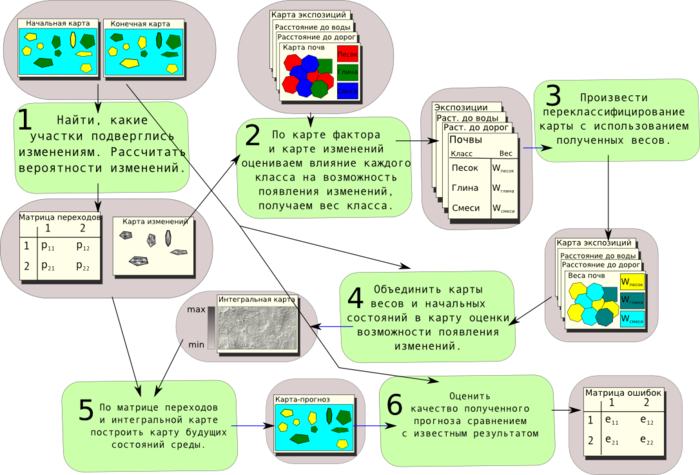
\includegraphics[width=0.9\columnwidth]{./introduction/img/MOLUSCE}
        \end{center}
    \end{figure}
\end{frame}
\note{
Про технологию модуля
}

